\documentclass{../mypaper}

\title{XY-plotter}
\author{Christian Klim Hansen \and Kristian Kjærgaard \and Nick Østergaard}
\date{\today}

\hypersetup{
  pdftitle={AceHigh, en (x,y)-plotter},
  pdfsubject={},
  pdfauthor={Christian Klim Hansen, Kristian Kjærgaard og Nick Østergaard},
  pdfcreator=LaTeX,
}

\pagestyle{Ruled}


\begin{document}

\begin{titlingpage}
  \maketitle
  
\includegraphics[width=\textwidth]{../logo/logo}

  \newpage

  \strut \vfill
  {
    \footnotesize
    \noindent Kristian Kjærgaard er megasej
  }

\end{titlingpage}

\frontmatter

\tableofcontents

\chapter{Forord}

% Terminologi, om kodeeksempler, rapportopbygning, kildehenvisning,
% referencer

\section{Om rapportens opbygning}

Rapporten er delt ind i fire hovedafsnit.

Afsnittet~\titleref{ch:indledning} på side~\pageref{ch:indledning}
beskriver de krav, plotteren skal overholde. Afsnittet giver et
udgangspunkt for at lave en løsning.

Delen~\titleref{prt:design} på side~\pageref{prt:design} diskuterer
forskellige løsninger til de krav, der er opstillet i
indledningen. Delen diskuterer mulige mekaniske, hardwaremæssige og
softwaremæssige løsninger og begrunder valget af den løsning, der
implementeres.

Delen~\titleref{prt:implementering} på
side~\pageref{prt:implementering} beskriver, hvordan den valgte
løsning realiseres og gennemgår i detaljer, hvordan løsningen
fungerer.

Afsnittet~\titleref{ch:afslutning} på side~\pageref{ch:afslutning}
samler op på vores projekt.  Afsnittet hænger sammen med
kravspecifikationen. Har vi opfyldt kravene? Hvad har vi lært?  Hvad
kunne vi gøre bedre?  \fixme{Anden formulering?}

Bilaget~\titleref{ch:bilag-rettelser-software} på
side~\pageref{ch:bilag-rettelser-software} indeholder rettelser til
dokumentationen af softwaredesignet og -implementeringen.


\section{Terminologi}

% Her skriver vi hvilken betydning forskellige ord har i
% rapporten. Hvad betyder fx software, MCU, plotter etc.

Med software menes den ekserkvering, der sker på mikroprocessoren i
plotteren. Når forkortelsen \enquote{MCU} nævnes, menes der selve
mikroprocessoren. MCU er en forkortelse for \textit{Micro Controller
  Unit}. Hardwarediagram er selve diagrammet over de elektroniske
kredsløb, mens printudlægget er selve det færdige kredsløb på
printkortet. Step og skridt bruges i flæng, når vi omtaler at en
stepmotor skifter position.  \fixme{Terminologi sektion renskrives!}

\fixme{grafikenheder skal nævnes}


\section{Angivelse af forfatter}

For at efterkomme et formelt krav er navnet på forfatteren til det
enkelte afsnit angivet i margin ved afsnittets begyndelse.


\section{Kilder}
Til skabelsen af plotteren, har vi selvfølgelig fået inspiration og
information fra andre kilder end os selv. Vi har derfor opstillet en
litteraturliste, som det ses på side ~\pageref{ch:litteratur}, med den
litteratur og de kilder vi har brugt.


\section{Takkeskrivelse}

% bl.a. tak til David Pedersen (Kjærgaards fætter) for vejledning om
% hvad? RepRap-fællesskabet (specielt fenn)
% Måske takke nogle af de kilder der er nævnt i litteraturlisten

Vi vil gerne rette en tak til alle, der på den ene eller anden måde
har bidraget til projektets tilbliven. Her særligt tak til
RepRap-fællesskabet\footnote{Se \url{http://www.reprap.org}.} og
\texttt{fenn}\footnote{Ukendt RepRap-fan mødt på IRC.} for
inspiration. Tak til David S. Pedersen for vejledning i forbindelse
med valg af dataformat. Tak til Roland Riegel\footnote{Se
  \url{http://www.roland-riegel.de}.} for GPL-software til SD-kort.

Tak til miljøet omkring den frie software. Fri tale, gratis øl og alt
det der\dots


%%% Local Variables: 
%%% mode: latex
%%% TeX-master: "../master"
%%% End:

\mainmatter

\chapter{Indledning}

% Note om hvad der skal stå i dette afsnit her.

Følgende rapport er skrevet i forbindelse med vores afsluttende
projekt i faget El-teknik.  Vi har fået udleveret tre mulige temaer,
hvor vi har valgt at arbejde med temaet: Robotteknologi, som omfatter
følgende:

\begin{itemize}
\item Udvikling af udstyr med funktioner af robotagtig karakter
\item Dette udstyr skal virke uden menneskelig indgriben
\end{itemize}

Vi ønsker, at opfylde disse krav ved at lave en plotter, som aflæser
data fra et SD-kort. Plotteren har til formål at tegne en figur på et
stykke A4-papir \fixme{Kjærgaard:referer til kravspecifikation}. Vi
har haft i alt 100 timer pr. person fordelt ud over 10 uger. Vi har
fået stillet 300 kr. pr. person til rådighed i dette projekt til fri
benyttelse, så længde at det har en tydelig relevans for vores
projekt. Samtlige indkøb skal godkendes af læreren.


\section{Overordnede produktkrav}

Vores produkt skal indeholde følgende elementer for at overholde
produktkravene:

\begin{itemize}
\item Der skal indgå mindst et elektrisk kredsløb med passive og
  aktive komponenter udover microcontrolleren
\item Der skal designes print layout vha. CAD
\item Der skal anvendes mindst én microcontroller
\item Der skal benyttes avancerede funktioner i microcontrolleren, som f.eks.:
  \begin{itemize}
  \item Interrupt
  \item Timer
  \item Tæller
  \item U(S)ART eller ADC
  \end{itemize}
\end{itemize}


\section{Kravspecifikation}

Vi vil lave en plotter, som opfylder følgende specifikationer:

\begin{itemize}
\item Plotteren skal tegne en figur, som vi har tegnet på computer
  \begin{itemize}
  \item Skal tegne på et stykke A4-papir
  \item Fungere uden at en computer er tilsluttet
  \item Læse data fra SD-kort
  \end{itemize}
\item Kunne forstå følgende elementer af HPGL:
  \begin{itemize}
  \item Rette linier
  \item Cirkler
  \end{itemize}
\item Anvende en AVR-processor
\item Bruge en pen til at tegne
  % \begin{itemize}
  % \item Bemærk at der ikke skal benyttes blyant eller kuglepen
  % \end{itemize}
\item Styre hastigheden af pennen meget præcist
  \begin{itemize}
  \item Med software skal vi gøre optimalt nytte af stepmotorenes præcision
  \end{itemize}
\item Kunne lave nødstop og restart med knapper
  % \item Vise status af tegneforløb på LCD-display eller med lysdioder
\item Kunne gå i nulstillingsposition (et sted hvor maskinen ved den
  så er) ved tryk på en trykknap
\item Den mekaniske konstruktion skal ligne figur\vref{fig:plotterskitse}
  \mnote{
    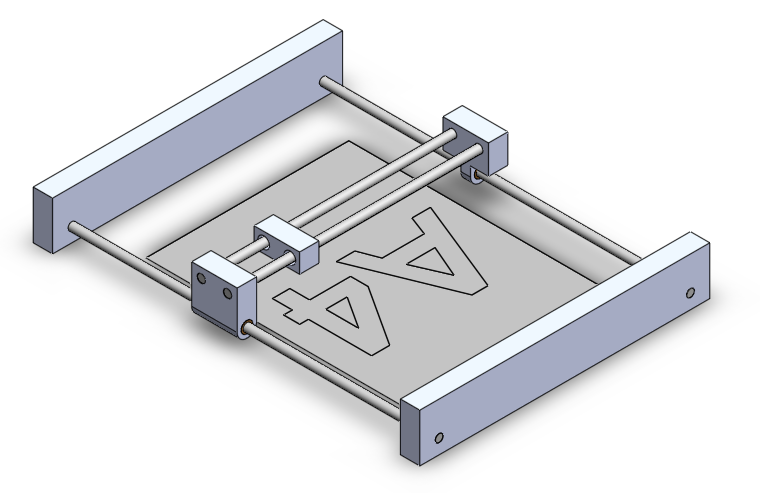
\includegraphics[width=\marginparwidth]{img/plotterskitse}
    \captionof{figure}{Skitse af konstruktion}
    \label{fig:plotterskitse}
  }
\item Bruge tandrem til at trække x- og y-akserne
  \begin{itemize}
  \item Tandrem er forbundet med stepmotor
  \end{itemize}
\item Pennen kan løftes og sænkes
\end{itemize}


\section{Terminologi}

% Her skriver vi hvilken betydning forskellige ord har i
% rapporten. Hvad betyder fx software, MCU, plotter etc.

Med software menes den ekserkvering, der sker på mikroprocessoren i plotteren.


\section{Om kodeeksempler i rapporten}

Alt software i vores projekt er udviklet med den frie GNU AVR C
Compiler\fixme{korrektur}, som virker på både Windows og Linux.

\fixme{Terminologi og Om kodeeksempler i rapporten bør nok være i Forord}

%%% Local Variables: 
%%% mode: latex
%%% TeX-master: "../master"
%%% End: 
\chapter{Brugervejledning}

% Note om hvad der skal stå i dette afsnit her.



%%% Local Variables: 
%%% mode: latex
%%% TeX-master: "../master"
%%% End: 

\part{Design}

\chapter[Design af mekanik]{Mekanik}
\mnote{Nick Østergaard}

% Her beskrives de overvejelser vi har haft omkring udformningen af
% vores mekanik.

I vores overvejeler omkring udformningen af vores produkt, så vi på
selve funktionen af produktet. Fordi vores produktet har til formål at
plotte en figur på et stykke A4-papir, så er det vigtigt, at
mekanikken er så slørfri som muligt. For at undgå slør har vi set på
placeringen af pennen, forskellige konstruktioner til akserne, og
hvilken metode vi vil bruge til at flytte akserne med.

Vi havde to forskellige forslag til udformningen glideren. De to
stænger, som pennen kører på, kunne enten være placeret vandret, som
ses på figur\vref{fig:glider}, eller lodret. Vi kom frem
til, at det, som ville resultere i mindst slør, var, hvis gliderne var
placeret vandret. Pennen styres af en stepmotor, som er placeret ude i
en af siderne.

\mnote{
  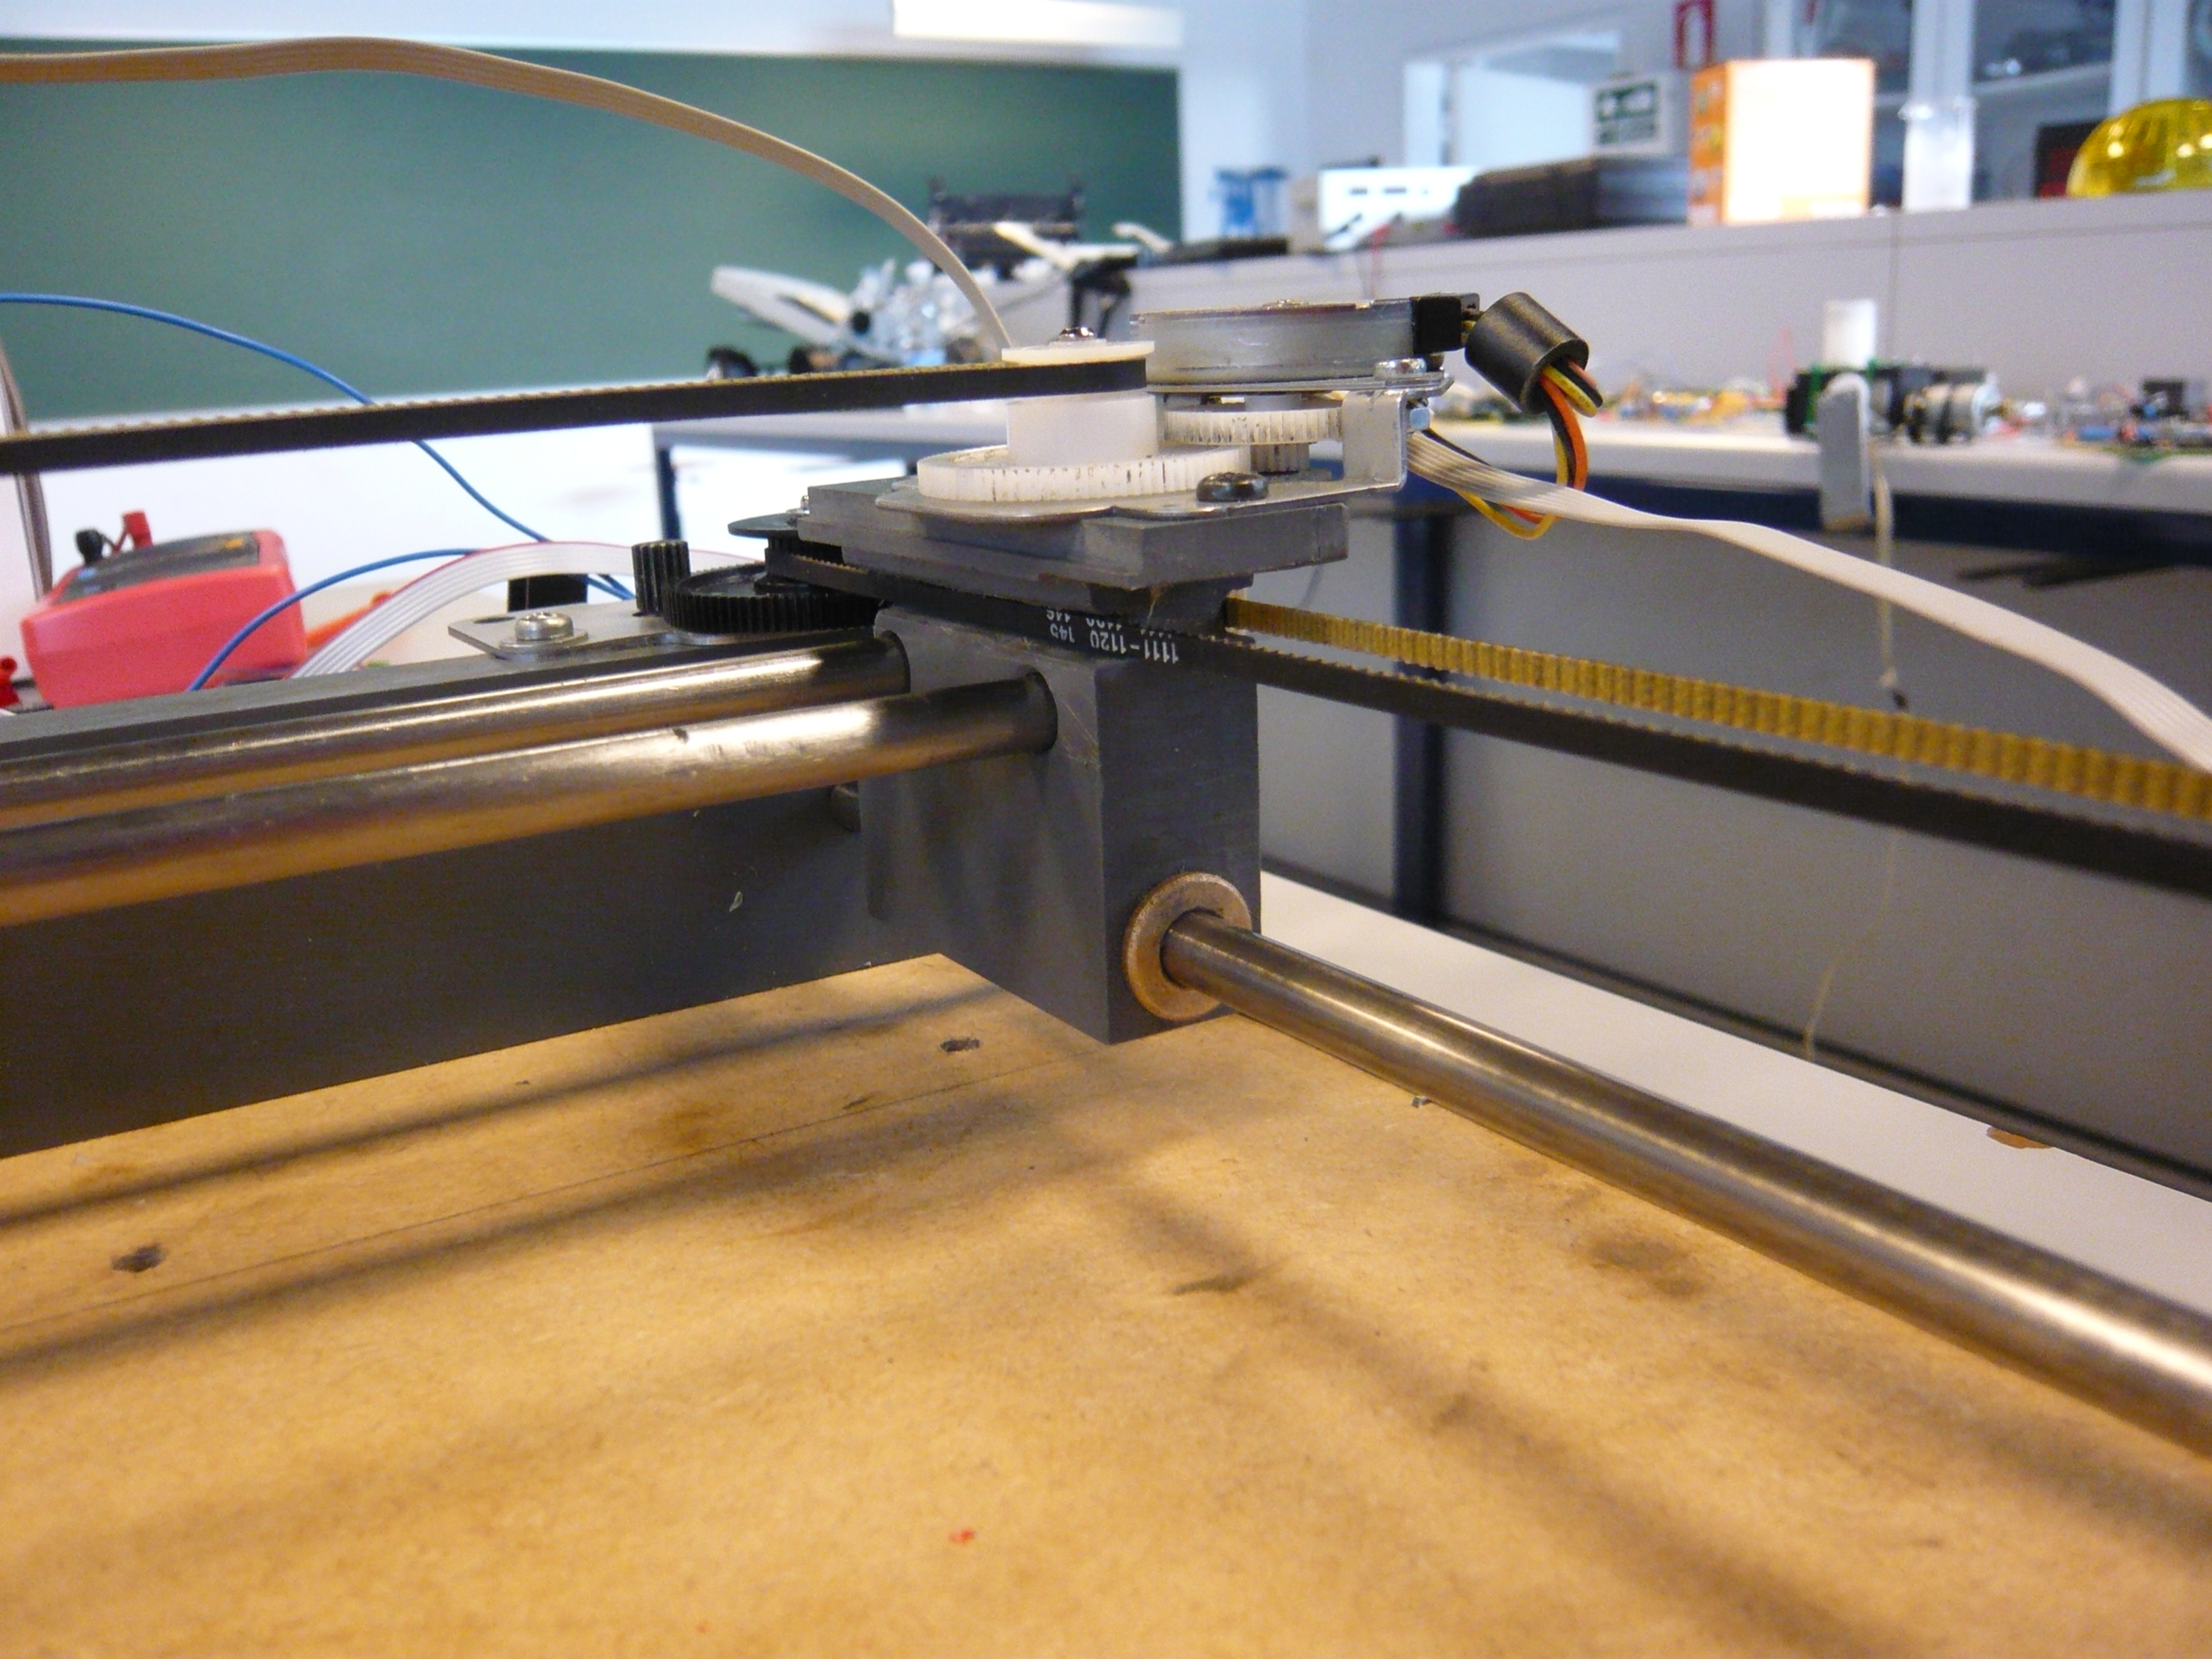
\includegraphics[width=\marginparwidth]{./img/glider}
  \captionof{figure}{Vandret glider}
  \label{fig:glider}
}

Et andet problem omkring slør var placeringen af stepmotoren, som skal
styre gliderne. Her kunne vi placere stepmotoren i midten af selve
konstruktionen eller ude i en af siderne. Hvis
stepmotoren blev placeret i midten af plotteren, så ville det først og
fremmest resultere i en større konstruktion, da stepmotoren skulle
placeres over glideren, men ligeledes ikke gøre meget for at hjælpe på
sløret. Hvis vi istedet placere stepmotoren i siden, som det vises i
afsnit~\vref{sc:stepmotor-driver}, så vil den være i
samme plan som glideren, hvilket ville gøre konstruktionen en del
mindre og samtidig hjælpe på sløret. Glideren ville da først bevæge sig,
når sløret er nogenlunde væk, hvilket giver anledning til en mere
præcis plotning.

Enkelheden af konstruktionen var ligeledes en essentiel del af vores
projekt, da vi har en begrænset periode, hvori vi kan udforme vores
produkt. Produktets størrelser var dog ikke under magen diskusion, da
det simplistiske skulle være en gennemtrængende del uden at have en
indvirkning på produktets funktionalitet. Gliderne samt glidelejrene er
lavet i stål for reduceret gnidningsmodstand. Vi bruger også olie til
yderligere at gøre modstanden mindre, og derved minske sløret.

\fixme{Omformuler dårlige formuleringer} \fixme{Billede med
  betegnelser med de forskellige komponenter på plotteren (tegnehoved,
  glider osv.)}

%%% Local Variables: 
%%% mode: latex
%%% TeX-master: "../master"
%%% End: 
\chapter[Design af hardware]{Hardware}
\label{ch:d-hardware}
\mnote{Nick Østergaard}

% Afsnittet skal indeholde information om vores hardware.
% Strømforsyning, motor drivere, MCU print, transducere m.m. Men kun
% hvad vi kan gøre, for at opfylde vores krav, ikke hvordan vi faktisk
% konstruerer det.

Med hensyn til hardwaren er der flere ting, der skal tages hensyn
til, hvilket er det, vi vil gøre i dette afsnit.


\section{Stepmotordriver}

Opgaven er at lave en plotter, hvilket kræver, at vi kan flytte en pen
i to retninger svarende til x- og y-akser i et plan. For at styre
disse to akser er det vigtigt, at vi nøjagtigt kan holde styr på, hvor vi
er. Til dette er stepmotor styring godt, da vi præcis ved, hvor vi er,
hver gang vi har taget et skridt.

I vores tilfælde bruger vi nogle stepmotorer fra et par
bordscannere. Motorerne er forskellig fra hinanden, da det er to vidt
forskellige scannere, de kommer fra. Da vi har to forskellige motorer,
som vi ikke kender specifikationerne på, har vi valgt, at lave et
driver print med adskilte kredsløb til hver motor. Vi opnår herved en
vis fleksibilitet, da vi på den måde kan have forskellig
forsyningsspænding til hver motor. Hvis vi havde lavet den med
sammenbyggede kredsløb, ville vi ikke kunne have forskellige
forsyningsspænding til hver motor, hvilket begge motorer måske ikke
vil køre optimalt ved.

Det skal dog lige nævnes, at den ene motor er en bipolar motor, mens
den anden er en unipolar motor. Vi vil dog styre begge motorer som
bipolare stepmotorer, fordi vi har nogle integrerede stepmotor
drivere til rådighed, som kun kan styre bipolare motorer.


\section{Sensorer}

Vi skal være i stand til at nulstille maskinens position i forhold til
vores koordinatsystem, fordi vi skal vide, hvor vi har vores
udgangspunkt.

For at opnå dette kan man gøre det, at man kører motorerne i retning
mod et nulpunkt, men kører længere end det faktisk er muligt at
køre. Det skal have til formål, at hovedet bliver trukket til
origo. Denne metode er dog ikke praktisk anvendelig, da man vil belaste
mekanikken og motorerne for meget og på den måde risikere at ødelægge
konstruktionen.

Vi vil derfor anvende nogle sensorer til at fastlægge en nulstillingsposition.
Vi kan anvende et par fotogafler, hvor vi fører
en mekanisk fane ind i. Maskinen kan så dedektere, hvornår der kommer
noget ind for sensoren, hvilket betyder, at vi ved, hvor vi er. Ud fra
hvilke signaler vi får fra de forskellige sensorer, så kan vi stoppe
maskinens bevægelse. Til sidst ved vi, at vi er i nulstillingspositionen (origo)
, altså at maskinen er nulstillet. Vi kan herefter begynde at anvende
maskinen. Det kræver selvfølgelig, at man placerer sensorerne, således
at mekanikken aldrig når at komme til sine yderpunkter, hvor den ikke
kan bevæge sig længere.


\section{SD-kort adapter}

Vi har i kravspecefikationen bestemt, at vi skal kunne styre maskinen
vha. data fra et SD-kort. Et SD-kort kan styres på forskellige måder:

\begin{itemize} \firmlist
\item{SPI mode (seperat serial ind eller serial ud)}
\item{Et-bit SD mode (seperat kommando og data kanaler samt et
    proprietært overførsels format)}
\item{Fire-bit SD mode (bruger ekstra forbindelser samt nogle
    ombyttede pins for at supportere fire bits bredde på parallel
    overførsel)}
\end{itemize}

Vi har valgt at kommunikere med SD-kortet via SPI-mode, da
\cite{web:captain-mmc} bruger dette og det er det simpleste jævnfør
ovennævnte som er fra \cite{web:sd-pinout}.

Som en følge af hvilken måde vi vælger at kommunikere med SD-kortet,
skal hardwaren understøtte funktionen. Der er dog ikke stor forskel imellem
SPI mode, som vi vil understøtte, og SD mode, som blot kræver to
forbindelser mere til SD-kortet. SPI er dog den simpleste
af de to.

SD-kortet opererer ved en spænding på 3,3V, derfor skal vi have en
seperat spændingsforsyning på 3,3V til kortet. Af samme grund er vi
nødt til at sænke spændingen fra vores MCU fra de 5V til omkring de
3,3V, før vi kan kommunikere med det. Vi kan opnå dette med en
spændingsdeler ved IO pinsene, der går fra MCU'en til SD-kortet. Når
signalet fra SD-kortet går høj, vil det givetvis være på 3,3V. Dette
er ikke de 5V, som vores MCU opererer ved, men det er ikke noget
problem, da det stadigvæk svarer til et højt signal for MCU'en.


\section{Tegnehoved}
\label{sc:d-tegnehoved}

Tegnehovedet er vores penholder,som sørger for, at vi kan hæve og sænke
pennen afhængig af, om vi skal tegne eller bare flytte pennen. Den kan
flyttes i to retninger (ad x- og y-aksen).


\section{Valg af mikroprocessor}
\label{sc:d-mikroprocessor}

Vi har til alle tidligere projekter brugt en AVR-processor af modellen
\texttt{atmega16}. Under udvikling af vores software til dette projekt
er vi blevet bekymret for den lille SRAM-hukommelse, som
\texttt{atmega16} indeholder.

Vi har lavet et andet mikroprocessorkort til en
\texttt{atmega128}. Denne har givet os rigelig med hukommelse, og den
har også flere IO-porte end de fire \texttt{atmega16} har. Det gør det
lettere at tilslutte andre enheder.

Vi bruger IO-porte til
\begin{enumerate} \firmlist
\item{kontrol af stepmotorer,}
\item{LCD-display,}
\item{statuslamper, knapper og til tegnehovedet,}
\item{SD-kort adapteren, og}
\item{ensorerne.}
\end{enumerate}

%%% Local Variables: 
%%% mode: latex
%%% TeX-master: "../master"
%%% End: 


\chapter{Software}

% Note om hvad der skal stå i dette afsnit her.


\section{Motorstyring}

\mnote{Kristian Kjærgaard skriver}

Dette afsnit diskuterer forskellige metoder til at styre tegnehovedets
placering.

Hastigheden for tegnehovedet er givet ved
\begin{align}
  v = \frac{\Delta x}{\Delta t}
\end{align}
hvor $v$ er hastigheden, $x$ er positionsændring og $t$ er
tidsændring. En præcis styring af hastighed kræver et præcist kendskab
til både positionsændring og tidsændring.

Den mindst mulige positionsændring er ét skridt med
stepmotoren\fixme{fælles: andet ord?} og kendskabet til denne er
tilstrækkeligt.

Følgende to afsnit diskuterer to forskellige metoder til at
\textit{time} motorerne.


\subsection{Motorstyring med indlagt forsinkelse}

En metode at styre timingen er ved at afvikle tidsberegningen på en
tråd med indlagt forsinkelse. Se
figur\vref{fig:motorstyring-indlagt-forsinkelse}.

\begin{figure}[htbp]
  \centering
  
\includegraphics[width=.7\textwidth]{../brugere/kjaergaard/motorstyring-indlagt-forsinkelse}
  \caption{Motorstyring med indlagt forsinkelse.}
  \label{fig:motorstyring-indlagt-forsinkelse}
\end{figure}

Ved denne type motorstyring er tiden $t$ mellem
skridtene\fixme{fælles: andet ord?} være givet ved
\begin{align}
  \Delta t &= t_e + t_d \nonumber \Rightarrow \\
  v &= \frac{\Delta x}{t_e + t_d}
\end{align}
hvor $t_d$ er den indlagte forsinkelse og $t_e$ er den tid det tager
at afvikle tidsberegningen. Da $t_e$ ikke kendes på
afviklingstidspunktet - og \textit{kan} variere fra afvikling til
afvikling afhængig af tallenes størrelse - er metoden upræcis ved høje
hastigheder. I figur\vref{fig:motorstyring-indlagt-forsinkelse-timing}
ses en situation, hvor størrelsen af $t_e$\fixme{kjærgaard: skriv
  afsnit færdigt, brug skitser fra egne notater}

\begin{figure}[htbp]
  \centering
  \vspace{3cm}
  \caption{Hastighed som funktion af forsinkelse for motorstyring med
    indlagt forsinkelse.}
  \label{fig:motorstyring-indlagt-forsinkelse-timing}
\end{figure}


\subsection{Motorstyring med afbrudt afvikling}

Alternativt kan motorerne times med afbrudt afvikling. Med en fast
fekvens tjekkes der, om det er tid til at flytte motorerne. Når der
ikke tjekkes om motorerne skal flyttes, beregnes det næste tidspunkt,
motorerne skal flyttes. Se
figur\vref{fig:motorstyring-afbrudt-afvikling}.

\begin{figure}[htbp]
  \centering
  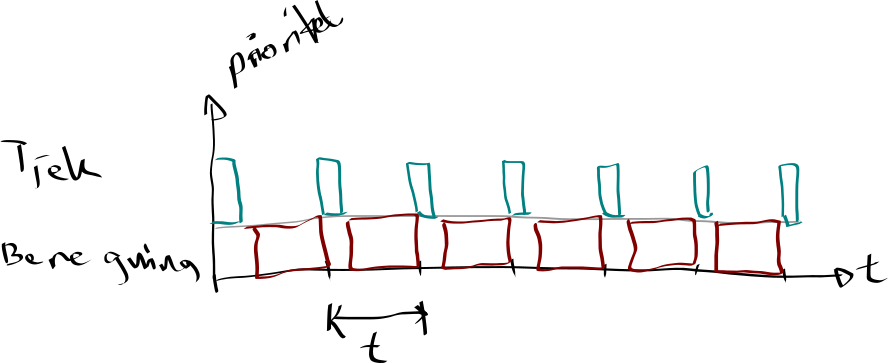
\includegraphics[width=.8\textwidth]{../brugere/kjaergaard/motorstyring-afbrudt-afvikling}
  \caption{Motorstyring med afbrudt afvikling.}
  \label{fig:motorstyring-afbrudt-afvikling}
\end{figure}

Den algoritme, der beregner hvilke tidspunkter, motorerne skal flyttes
på, afvikles hele tiden. Når det er tid til at tjekke, om vi har
overskredet et tidspunkt, afbrydes afviklingen af
beregningsalgoritmen, og tjekkeralgoritmen afvikles. Når
tjekkeralgoritmen\fixme{fælles: andet ord!} er afviklet, fortsættes
afviklingen af beregningen af tidspunkter.

Med denne metode kendes mindst mulige forsinkelse $t$, og vi har hvad
vi efterspørger. Forskellige hastigheder opnås ved at udelade at
flytte motorerne på alle tidspunkter (se
figur\vref{fig:motorstyring-afbrudt-afvikling-hastighed}), og
præcisere styring af hastigheden opnås ved at afvikle
tjekkeralgoritmen med større frekvens. \fixme{kjærgaard: anden
  formulering}

\snote{
  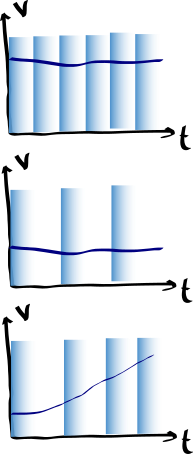
\includegraphics[width=\marginparwidth]{../brugere/kjaergaard/motorstyring-afbrudt-afvikling-hastighed}
  \captionof{figure}{Eksempel på høj hastighed, lav hastighed og
    acceleration ved motorstyring med afbrudt afvikling.}
  \label{fig:motorstyring-afbrudt-afvikling-hastighed}
}

Løsningen forudsætter, at
\begin{itemize}
\item dataene fra algoritmen, der beregner tidspunkter, kan opbevares
  i en kø,
\item der er data i køen, når tjekkeralgoritmen har brug for data at
  tjekke mod, og
\item beregningsalgoritmen kan afvikles så hurtigt, at der lægges data
  i køen hurtigere end tjekkeralgoritmen gennemgår dem.
\end{itemize}

I værste tilfælde skal behandlingsalgoritmen
\begin{itemize}
\item indlæse data fra datakilden,
\item fortolke dataene og
\item beregne tidspunktet
\end{itemize}

Med en taktfrekvens på 16 MHz


\section{HP-GL -- Hewlett-Packard Graphics Language}

Når man skal vælge, hvilket format man vil bruge, når man laver en
plotter, så er der en del ting at tage hensyn til. Der findes mange
forskellige standarder, som kan anvendes og en af disse standarder er
HPGL, som vi benytter os af.

Når man skal vælge, hvad man vil bruge, så er det vigtigt at se på
fordele og ulemper. Vi kunne i princippet godt udvikle vores eget
plotterformat, men dette vil både være meget tidskrævende, og
samtidigt vil det være svært at få implementeret, da vores format ikke
er en standard, og derfor er der ikke noget som direkte virker med
det. Derfor er HPGL velegnet i vores projekt, da det er mere
virkelighedsnært at benytte en standard, som allerede er konstrueret
som et plotterformat, samtidig med at det kan anvendes af forskellige
applikationer (andre CAD programmer). Der er heller ikke mange ulemper
tilknyttet til brugen af HPGL som plotterformat. Det vil dog tage lang
tid at implementere det hele, hvilket vi dog heller ikke gør. Vi
kommer f.eks. ikke til at benytte os af pin-skrift og en del andre
ting, men disse problemer er relativt lette at komme udenom.

Når man betragter HPGL som et plotterformat, så betyder det, at den
indeholder mange forskellige kommandoer med hver deres funktion. Det
kan tage lang tid at sætte sig ind i alle disse ting, men hvis man har
forståelse for, hvilke funktioner vi evt. kommer til at bruge i vores
projekt, vil det selvfølgelig lette indlæringsarbejdet en del.

Følgende er en tabel over vores overvejelser omkring fordele og
ulemper ved brugen af eget dataformat samt fordele og ulemper ved
brugen af HPGL:

\fixme{Her indsættes tabel over fordele og ulemper ved eget
  dataformat. Denne tabel eksistere allerede}

Dette betyder, at der findes ingen software, der kan håndtere
formatet. Dette betyder at vi selv skal skrive den software, som er
uden for rammer af dette projekt. Derfor leder vi efter en
eksisterende standard.

\fixme{Her indsættes tabel over f og u ved HPGL}

Dette betyder, at HPGL er meget velegnet til brug i vores projekt, da
formatet er veldokumenteret, afprøvet og anvendt industrielt til
specielt plottere, hvilket vores eget selvfølgelig også ville være, og
der finde allerede software, som kan håndtere formatet til forskel fra
vores eget. Implementeringstiden vil dog være en del længere, da
niveauet er sat fra starten, hvilket medfører en del ubenyttede
funktioner.


\section{Koordinatsystem}

% Skriv om koordinatsystemet

Vi arbejder med skærmkoordinater (se
figur\vref{fig:skaermkoord}). HP-GL (se
softwaredesignafsnit\fixme{kjærgaard:lav henvisning}) er formateret i
skærmkoordinater (og ikke Euklidiske koordinater?\fixme{tjek navn}),
og internt i softwaren (se igen
softwareafsnit\fixme{kjærgaard:henvisning}) kan en konvertering
springes over ved at bruge skærmkoordinater.

\snote{
  
\includegraphics[width=\marginparwidth]{../brugere/kjaergaard/skaermkoordinater}
  \captionof{figure}{Skærm\-koor\-dinater. Der arbejdes med
    skærmkoordinater i plotteren.}
  \label{fig:skaermkoord}
}


\section{Timing \& Buffer}

I afsnittet om mekanik lå fokus meget på nøjagtigheden af vores
produkt. Vi vil her diskutere, hvordan vi vil opnå denne nøjagtighed.

Vi har diskuteret to løsninger. Den ene forgår ud af en såkaldt tråd,
hvor vi udfører og holder pause, udfører og holder pause. Dette giver
dog anledning til en forsinkelse. Dette kan ses på figur\fixme{indsæt
  figur af trådløsning}.  Da vi ikke kan bestemme forsinkelsen i
praksis, så er denne løsning ikke optimalt til vores projekt.

Vi kom herefter frem til en løsning, hvor vi benytter os af en buffer,
som man kan læse mere om under afsnittet Software under
Implementering. Her udføres instruktionerne, som er samlet i bufferen
sammen med et tidspunkt, når dette tidspunkt er overskredet. Der skal
altså jævnt udføres et tjek, som den såkaldte deadline er
overskredet. Imellem disse tjek kan bufferen få data.

Der er dog problemer, som vi skal tage højde for, når vi bruger en
buffer. F.eks. må hastigheden af outputtet ikke overskride
hastigeheden hvormed bufferen får data fra HPGL. Sagt mere simpel, så
må bufferen aldrig tømmes helt. Hvis dette sker, så har bufferen ikke
nok information eller jobs til motorstyringen, hvilket medfører en
overskrides af vores deadline, svarende til det tidspunkt vi skal have
udført vores funktion. Afstanden imellem to tjek skal skal således
være stor nok, så bufferen har tid til at modtage data. Dataen kommer
som sagt fra HPGL, som har behandlet information fra SD-kortet. Dette
ses illustreret i figur\fixme{Illustration som viser overførsel af
  data fra SD-kort osv.}.

Vi skal også tage højde for, at bufferen ikke nødvendigvis bliver
fyldt før hvert tjek. Dette giver anledning til et interrupt, hvor
opfyldningen af bufferen stoppes og tjekket udføres. Efter tjekket
genoptages opfyldningen af bufferen. Brugen af en buffer har den
fordel, at hastigheden af output er nogenlunde konstant. Diagrammet
over brugen af en buffer kan ses i figur\fixme{indsæt figur over
  bufferforløb}.



\section{Valg af programmeringssprog}

Softwaren skrives i C og \Cpp.

C bruges i moduler, hvor sproget uden videre er tilstrækkeligt. Dette
vil typisk være lavniveaumoduler, og her er C fordelagtigt, fordi det
giver større kontrol.

\Cpp\ bruges i moduler, hvor det er fordelagtigt at bruge
\Cpp-speficikke elementer (f.eks. generisk programmering\fixme{note om
  dette?}). Moduler, der afhænger af moduler skrevet i \Cpp, vil
typisk også være skrevet i \Cpp.

Alle C-moduler er kompatible med \Cpp, og alle \Cpp-moduler er så vidt
muligt kompatible med C. Uønskede sideeffekter af \Cpp\ forsøges
undgået (\fixme{eksempler her!}). \Cpp\ bruges ikke objektorienteret.

\section{Matematikken bag}

Forholdet imellem tiden det tager at tegne linjen og tiden til et
punkt på linjen med $x$-koordinatet er lig forholdet imellem det givne
punkts x-koordinat og forskellen imellem start- og slutkoordinat $\Delta x$:

\begin{align}
\frac{t}{\Delta t} &= \frac{x}{\Delta x} \Rightarrow x(t) = \Delta x \times \frac{t}{\Delta t}
\end{align}

Den generelle formel for tiden $t$, det tager at tegne linjen, er lig:
\begin{align}
v &= \frac{L}{\Delta t} \Rightarrow \Delta t= \frac{L}{v}
\end{align}

Hvilket betyder, at vi kan kombinere (5.1) og (5.2):
\begin{align*}
\frac{t \times v}{L} &= \frac{x}{\Delta x}
\end{align*}

Ved isolering af tiden $t$ får vi at:
\begin{align}
t = \frac{x}{\Delta x} \times \frac{L}{v}
\end{align}

Længden af linjen $L$ er givet ud fra pythagoras læresætning:
\begin{align*}
L &= \sqrt{\Delta x^2+\Delta y^2}
\end{align*}

Forholdet imellem $x$ og $\Delta x$ kan beskrives som forholdet imellem step $n$ og total antal steps $\Delta n$:
\begin{align}
\frac{x}{\Delta x} = \frac{n}{\Delta n}
\end{align}

Indsættes dette i (5.3) får vi et udtryk for tiden $t$, som afhænger af step $n$:
\begin{align}
t &= \frac{n}{\Delta n} \times \frac{L}{v}
\end{align}

Step $n$ kan findes ved brug af følgende formel:
\begin{align}
n &= x \times \eta_x \qquad n \in{R}
\end{align}

Formlen fremkommer af vores definition på $\eta$, som er:
\begin{align*}
\eta_x = \frac{n}{x}
\end{align*}

Ud fra formlen fremgår det, at $\eta$ har enheden $\frac{steps}{mm}$.
Standardenheden, som er givet fra HPGL, er 0,025mm, altså en $\frac{1}{40}mm$


%%% Local Variables: 
%%% mode: latex
%%% TeX-master: "../master"
%%% End:

\part{Implementering}

\chapter[Implementering af mekanik]{Mekanik}

% Note om hvad der skal stå i dette afsnit her.
% Kort afsnit om hvordan vi har lavet vores produkt ud fra vores overvejelser

Figur \fixme{Indsæt figur over færdigt produkt} viser vores færdige produkt.
Udformningen af produktet tager udgangspunkt i vores overvejelser i design-afsnittet.
Man ser ud fra figuren, at akserne styres af to stepmotor, som er henholdsvis uni- og bipolar.
Vi startede med at lave basen for vores produkt. Her tog vi udgangspunkt i at vi skulle kunne
tegne på et stykke A4-papir. Yderligere har vi brug for plads til vores hardware, som styrer
stepmotorerne. Herefter blev gliderne og deres respektive dele lavet og sat sammen med basen,
som det fremgår af figuren. Vi havde brug for en holder til pennen, som passede med gliderne,
så det var naturligt, at lave denne i den afsluttende del af produktionsforløbet. Bemærk ud
fra figuren, at vi også bruger glidelejre for at reducere modstanden imellem glidere og "klods",
og derved give mindre slør.

\section{Tegnehovedet}\fixme{Under mekansik}
Tegnehoved er i afsnittet~\vref{sc:d-tegnehoved} beskrevet som en
penholder. Vores tegnehoved er konstrueret som det ses på
figur~\vref{fig:tegnehoved-skitse}.

På en glider, er der monteret en trækmagnet, som er forbundet mekanisk
til en arm der holder pennen. Armen holdes oppe af en fjeder. Når man aktiverer trækmagneten, vil 

\begin{figure}[htbp]
  \centering
  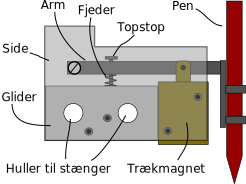
\includegraphics[width=7cm]{./img/tegnehoved-skitse}
  \caption{Skitse af tegnehoved}
  \label{fig:tegnehoved-skitse}
\end{figure}

\mnote{
  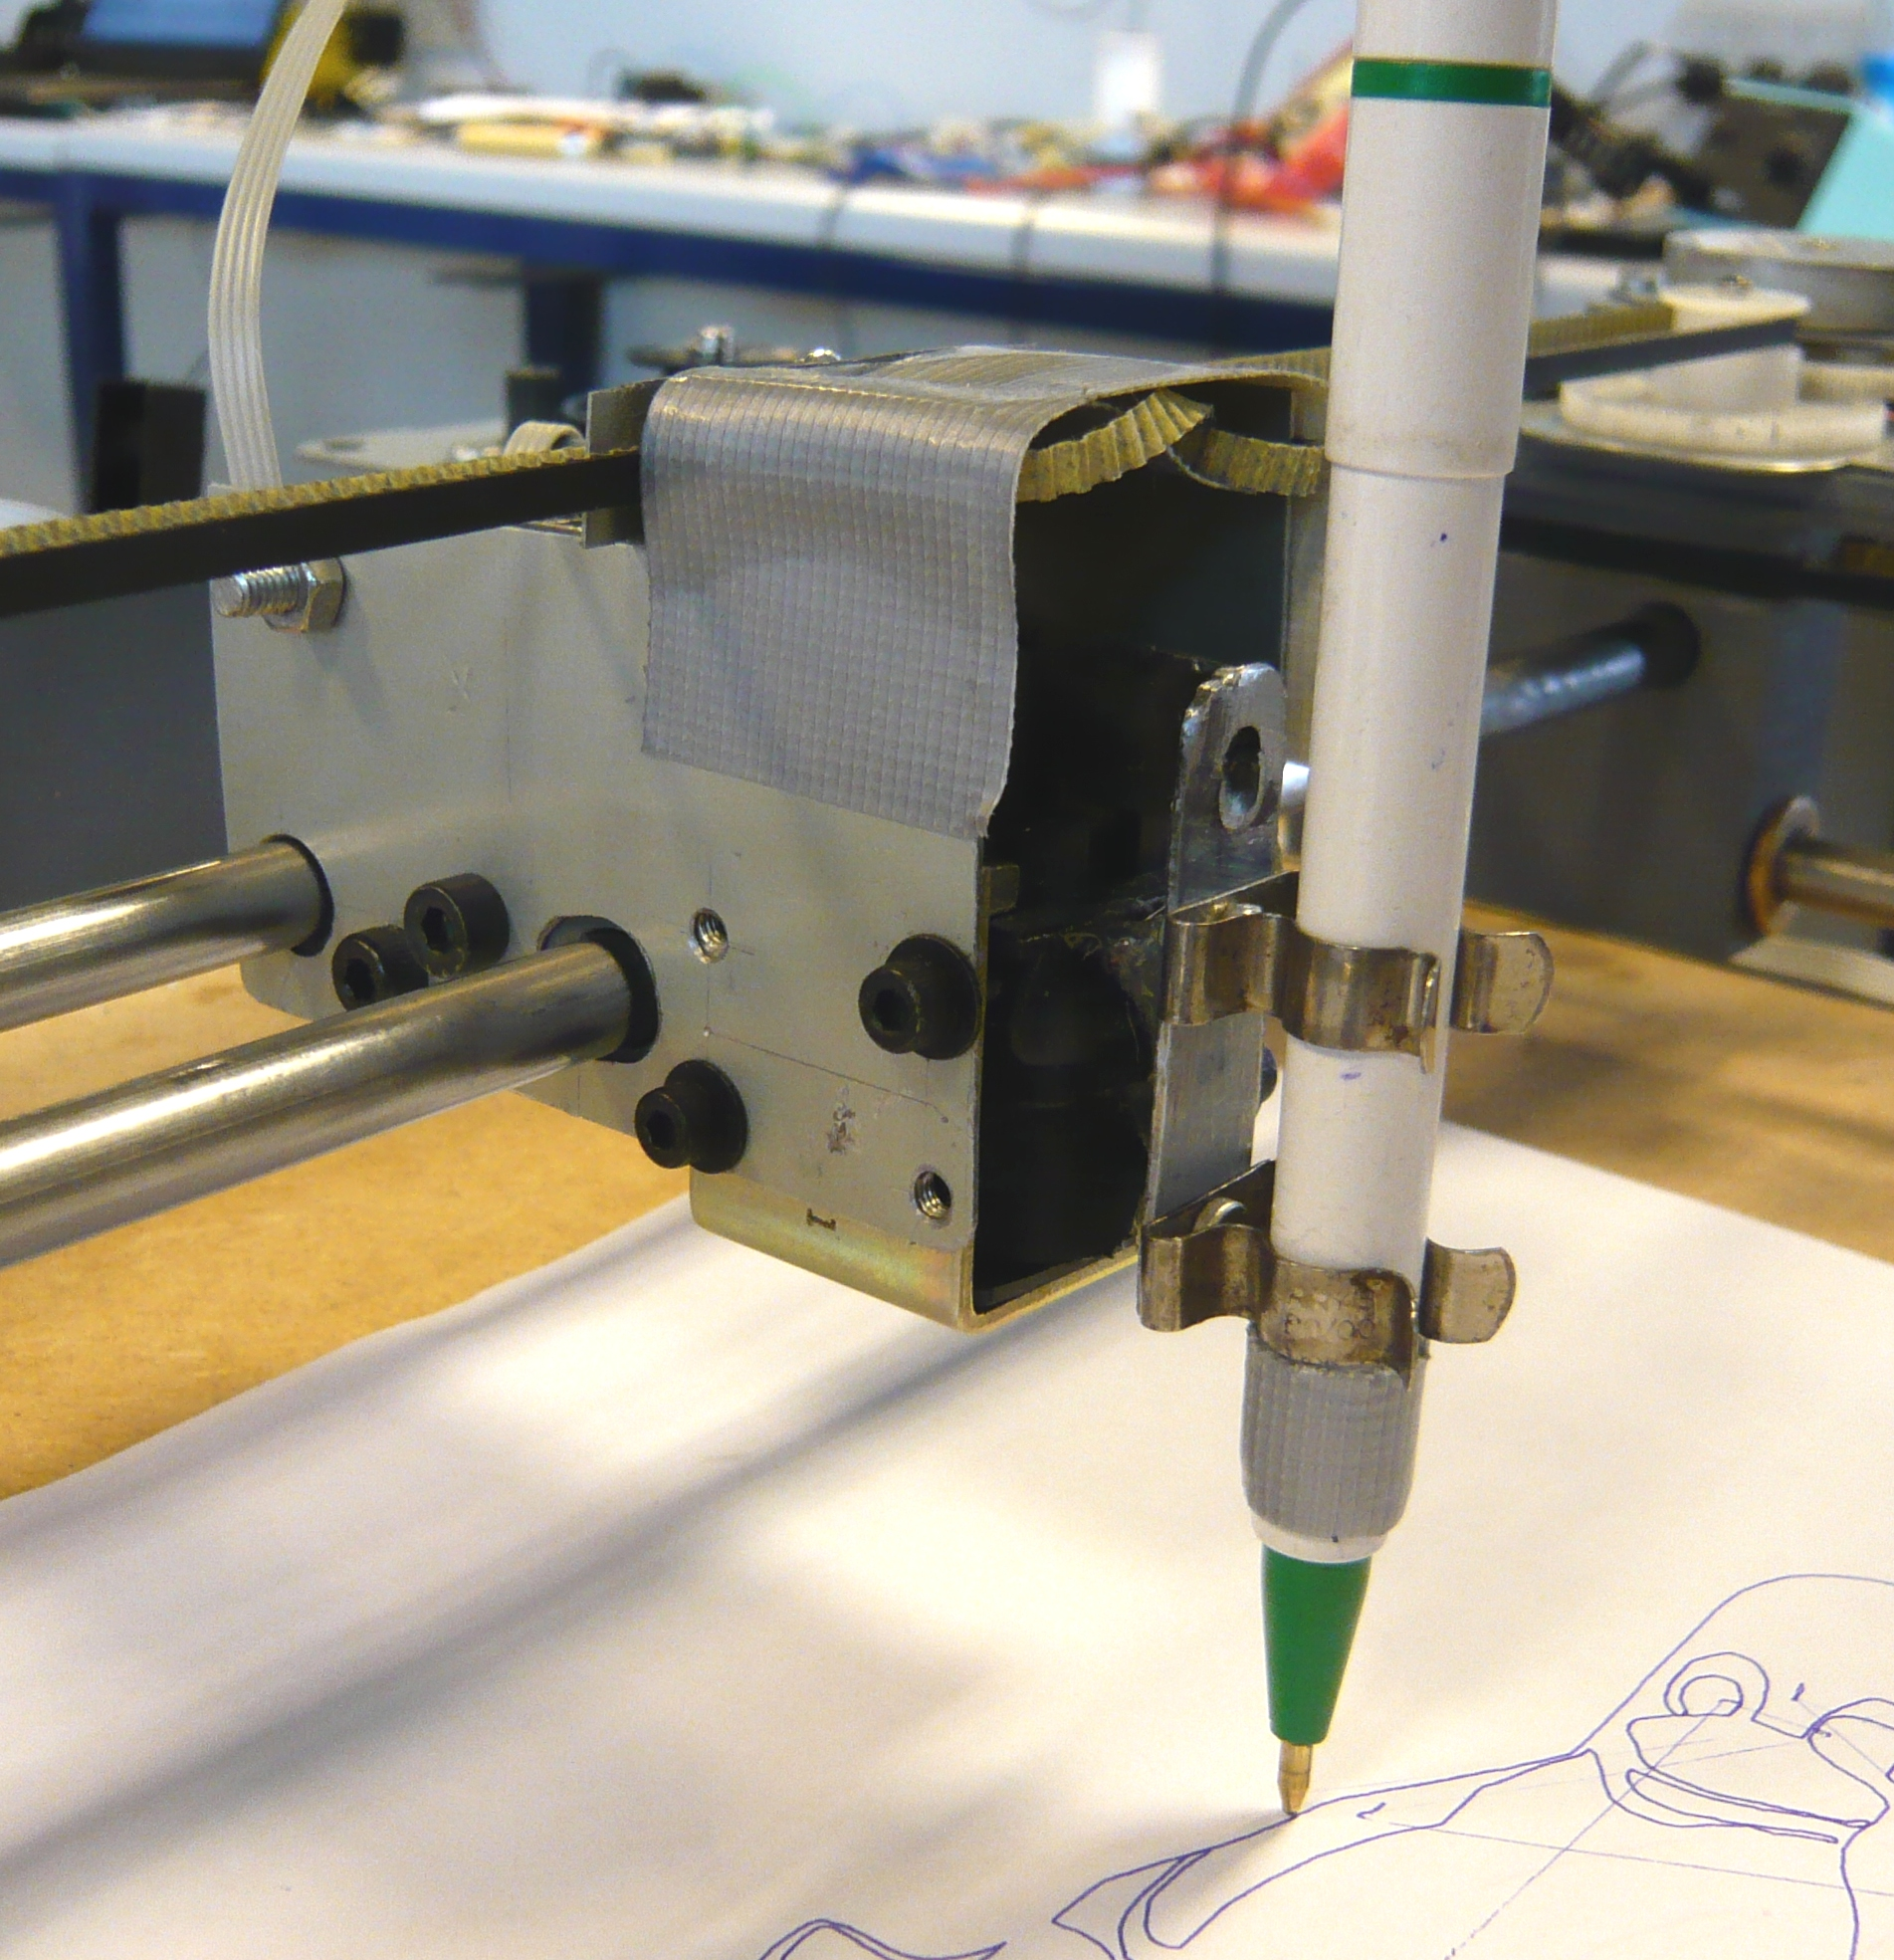
\includegraphics[width=\marginparwidth]{./img/tegnehoved}
  \captionof{figure}{Tegnehovedet i dets reele form}
  \label{fig:tegnehoved}
}

%%% Local Variables: 
%%% mode: latex
%%% TeX-master: "../master"
%%% End: 
\chapter[Hardwareimplementering]{Hardware}

% Note om hvad der skal stå i dette afsnit her.

\section{Transducer}
\fixme{delkredskøb til gaffelsensorerne}

%%% Local Variables: 
%%% mode: latex
%%% TeX-master: "../master"
%%% End: 
\chapter[Implementering af software]{Software}

% Note om hvad der skal stå i dette afsnit her.


\section{Oversigt over softwaren}
\mnote{Kristian Kjærgaard}

% Her skriver vi hvordan softwaren er struktureret - se figuren nedenfor.

Softwaren er struktureret som vist i
figur\vref{fig:software-oversigt}. Dataføderen leverer data til den
del af softwaren, der behandler HPGL. Dataen kommer fra et
SD-kort. HPGL-behandleren sender instruktioner videre til den del af
motorkontrollen, der afvikles når der er tid. Denne del sætter
instruktioner i kø til realtidsdelen.

Realtidsdelen af motorkontrollen behandler de instruktioner, den anden
del af motorkontrollen har sat i kø og styrer stepmotorer m.m. efter
disse instruktioner. Realtidsdelen af motorkontrollen har ansvar for,
at hastigheden af tegnehovedet kan styres præcist.


\begin{figure}[htbp]
  \centering
  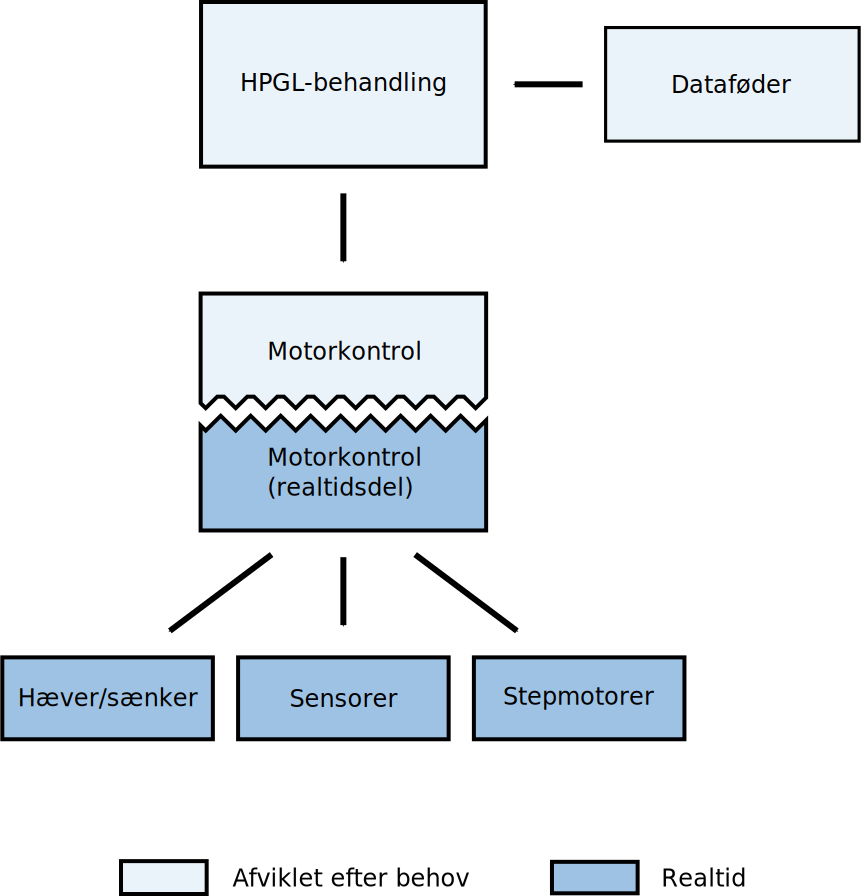
\includegraphics[width=.75\textwidth]{../brugere/kjaergaard/software-oversigt}
  \caption{Oversigt over softwaren. De lyseblå dele afvikles, når der
    er tid til det. Når det er tid til at afvikle de mørkeblå områder,
    afbrydes afviklingen af de lyseblå.}
  \label{fig:software-oversigt}
\end{figure}


\section[Dataføder (med SPI og SD-/MMC-kort)]{Dataføder}

% Hvordan virker dataføderen (herunder buffer, spi og sd/mmc)?

Dataføderen leverer data til HPGL-motoren og håndterer de
underliggende moduler, der indeholder data.

Dataføderens skal
\begin{itemize} \firmlist
\item levere data til HPGL-motoren og sørge for at denne ikke løber
  tør for data\fixme{bliv enig om terminologi}
\item stille et ensartet API\footnote{Application Programming
    Interface, programmeringsbrugerflade; betegnelse for struktur og
    navngivning for funktioner, variable, strukturer, klasser
    etc. brugt til programudvikling.}\fixme{brug evt. wikis
    formulering af api} til rådighed uafhængig af underliggende modul,
  således at det overliggende modul er uafhængig af det modul, der
  indeholder data - se figur\vref{fig:datafeeder-uniform-api}
\item håndtere fejl for underliggende moduler
\end{itemize}

\mnote{
  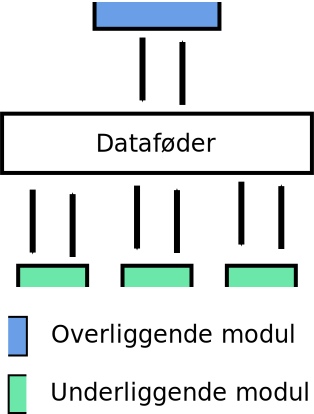
\includegraphics[width=\marginparwidth]{../brugere/kjaergaard/datafoeder-uniform-api}
  \captionof{figure}{Data\-føderen skal stille et ensartet API til
    rådighed.}
  \label{fig:datafeeder-uniform-api}
}

En oversigt over funktionsfordelingen\fixme{andet ordvalg} i
dataføreren\fixme{andet ordvalg} kan ses i
figur\vref{fig:software-spi-sd-oversigt}.

\begin{figure}[htbp]
  \centering
  \includegraphics[width=\textwidth]{../brugere/kjaergaard/datafeeder-oversigt}
  \caption{Diagram over funktionsfordeling i dataføderen}
  \label{fig:software-spi-sd-oversigt}
\end{figure}

Kommunikationen med SD-kortet foregår gennem SPI'en\fixme{afsnit skal
  skrives færdig}. Et eksempel på en forespørgsel med tilhørende svar
kan ses i figur\vref{fig:software-spi-sd-handling}.

\begin{figure}[htbp]
  \centering
  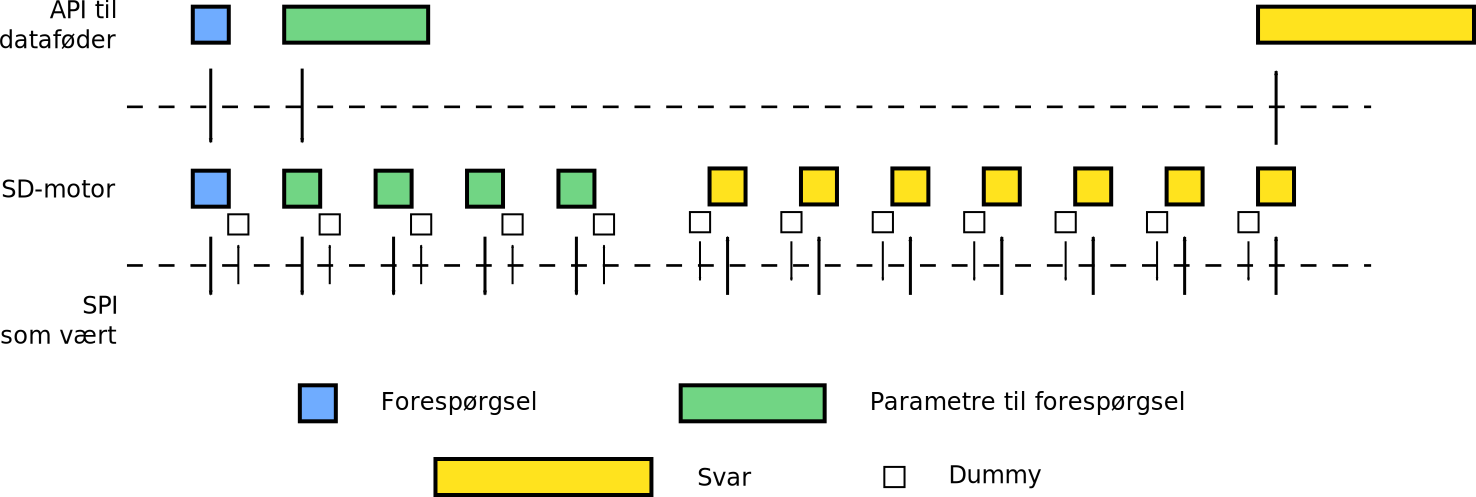
\includegraphics[width=\textwidth]{../brugere/kjaergaard/datafeeder-handling}
  \caption{Handlingdiagram ved kommunikation med SD-kortet}
  \label{fig:software-spi-sd-handling}
\end{figure}


\section{HPGL-behandleren}

\mnote{Christian Klim Hansen}

% Hvordan virker den del, der fortolker og behandler HPGL?
HPGL er et dataformat, som indeholder adskillige forskellige
instruktioner med forskellige parametre (se
afsnit\vref{sc:idn-ins-param}) . Vi benytter os ikke af samtlige
instruktioner, men blot et lille udvalg med udgangspunkt i vores
kravspecifikation.  I projektet anvender vi følgende instruktioner:

\begin{itemize} \firmlist
\item \texttt{PU} Pen Up - bruges til at hæve
\item \texttt{PD} Pen Down - bruges til at sænke pennen
\item \texttt{PA} Plot Absolut - se afsnit\vref{sc:relativ-absolut}
\item \texttt{PR} Plot Relative
\item \texttt{CI}  Plot Circle - se afsnit\vref{sc:matematik-cirkel}.
\end{itemize}

HPGL bruger oprindeligt bogstaver, tal og symboler (komma, punktum
osv.) til at identificere instruktioner, men som det fremgår af næste
afsnit, så anvender vi kun bogstaver i vores identifikation.

\subsection{Identifikation af instruktioner og parametre}
\label{sc:idn-ins-param}
\mnote{Kristian Kjærgaard}

% Her skriver vi hvordan vi identificerer instruktioner og parametre i
% datastrømmen

HPGL-behandleren identificerer instruktioner og parametre på
datastrømmen med en \textit{parser}. Databehandleren består af en
markør og pladsholdere til instruktioner og parametre.

Parseren er \textit{byte}-orienteret og kan kun se én byte ad gangen,
se figur\vref{fig:hpgl-parser-iden}. Afhængig af denne bytes værdi
gemmer parseren byten i en pladsholder og indlæser den næste byte for
at sætte kæden sammen til instruktioner eller parametre til
instruktioner.

% floaten ligger muligvis for lavt
\snote{
  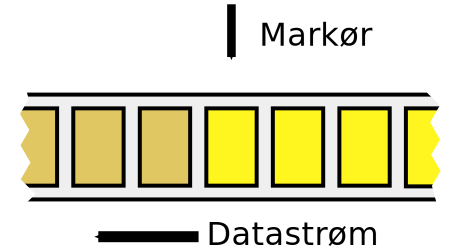
\includegraphics[width=\marginparwidth]{../brugere/kjaergaard/datafoeder}
  \captionof{figure}{Markøren på datastrømmen i HPGL-behandlerens
    identifikation af instruktioner på datastrømmen}
  \label{fig:hpgl-parser-iden}
}

Hvis byten ikke har en værdi, parseren forstår, flyttes markøren
videre til næste byte, således at den byte, markøren peger på, ikke er
fortolket.

Hvis byten er et bogstav, peger markøren på første byte i en
instruktion. Den næste byte indlæses og de to byte sættes sammen til
en instruktion.

Hvis byten er et tal eller punktum (.), peger markøren på første byte
i en talparameter. Der indlæses og gemmes bytes indtil den indlæste
byte ikke er et tal eller punktum. Når den indlæste byte ikke er et
tal eller punktum, konverteres de indlæste bytes til et tal.

Se afviklingsdiagrammet for parseren i
figur\vref{fig:hpgl-parser-afvikling}. Parseren understøtter ikke
andre parametre end talparametre.

\begin{figure}[htbp]
  \centering
  \subfloat[Afviklingsdiagram for parserens instruktionsidentifikation.]{
    \includegraphics[width=.30\textwidth]{../brugere/kjaergaard/hpglparser-ins}
  }
  \qquad
  \subfloat[Afviklingsdiagram for parserens parameteridentifikation.]{
    \includegraphics[width=.60\textwidth]{../brugere/kjaergaard/hpglparser-param}
  }
  \caption{Afviklingsdiagrammer for HPGL-parseren}
  \label{fig:hpgl-parser-afvikling}
\end{figure}


\subsection{Relative og absolutte koordinater samt grafikenheder}
\label{sc:relativ-absolut}
\mnote{Christian Klim Hansen}

Indenfor HPGL bruger man relative og absolutte koordinater. Absolut
plotning indeholder to parametre, X og Y. X og Y er absolutte værdier,
altså kan de ikke være negative, som måles enten i en brugerdefineret
enhed eller grafik enheder (0,025mm). Absolut plot bruges, når man vil
flytte pennen til en bestemt koordinat set fra origo $(0, 0)$. Ligesom
med cirklen, så plottes kun en linie, når pennen er nede.

\mnote{
  
\includegraphics[width=\marginparwidth]{./img/relativ-absolut}
  \captionof{figure}{Eksempel på relativ og absolut linie}
  \label{fig:relativ-absolut}
}

Relativ plotning indeholder ligeledes to parametre, x og y. x og y er
relative værdier til den nuværende position, altså kan de godt være
negative. Relativ plotning måles ligesom absolut. Relativ plotning
bruges, når man vil lave serie af linier i række, da man her tager
udgangspunkt i den forrige linies
slutpunkt. Figur\vref{fig:relativ-absolut} viser et eksempel på
relative og absolutte linier.

\subsection{Behandling af cirkel}
\label{sc:matematik-cirkel}

Vi kender cirklens radius $r$, kordevinklen $c$ samt startkoordinater
$(x, y)$. Det første koordinat kan ud fra en hurtig analyse derfor let
findes:
\begin{align*}
P_0(x, y)=(r, 0)
\end{align*}

\mnote{
  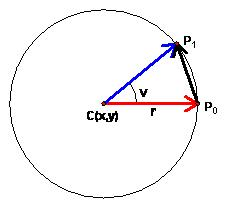
\includegraphics[width=\marginparwidth]{./img/cirkel}
  \captionof{figure}{Cirkel}
  \label{fig:cirkel-tegning}
}

Dette er tilfældet, da vinklen $w$ er $0\degree$.

Næste koordinat ligger i en vinkel $w$, som svarer til kordevinklen
$c$, altså har vi lagt en kordevinkel til de $0\degree$. Ved brug af
cosinus og sinus samt radius $r$ kan vi bestemme det næste koordinat:
\begin{align}
P_1(x, y)&=(\cos(w)\times r, \sin(w)\times r) \Rightarrow \nonumber \\
P_1(x, y)&=(\cos(c)\times r, \sin(c)\times r) \label{eq:8.1}
\end{align}
 
Denne formel kommer ud fra grundlæggende trigonometri:
\begin{align*}
\cos(v) &= \frac{x}{r} \Rightarrow x = \cos(v)\times r \\
\sin(v) &= \frac{y}{r} \Rightarrow y = \sin(v)\times r
\end{align*}
 
Formlen \vref{eq:8.1} kan omskrives, så den gælder et vilkårligt punkt
på cirkelperiferien:\fixme{denne henvisning er usikker}
\begin{align}
P_n(x, y)=(\cos(n\times c)\times r, \sin(n\times c)\times r)
\end{align}

Vi betragter en cirkel med en radius på 5cm og en kordevinkel på
$3\degree$. Første koordinat er således:
\begin{align*}
P_0(x, y)&=(\cos(0\times 3\degree)\times 5 , \sin(0\times 3\degree)\times 5)=(5, 0) \\
\end{align*}

Vi ser, at dette passer i overensstemmelse med første
udsagn. Vha. ovenstående formel kan vi blot lægge en til $n$ hver gang
funktionen er udført. Dette skal den blive ved med indtil vinkel
overskrider $360\degree$.


Der opstår dog et problem, hvis vinklen ikke går op i $360\degree$,
såsom vinklen $7\degree$. $51\times 7\degree = 357\degree \Rightarrow
\textup{rest} = 3\degree$. Overskrider vinklen de $360\degree$, har vi to
muligheder:
\begin{itemize} \firmlist
\item Funktionen afsluttes uden at slutte cirklen
\item Funktionen ændres, så optegningen fortsætter til udgangspunktet $P_0$
\end{itemize}
Det skal også nævnes, at HPGL tegner uanset om pennen er oppe eller
nede, hvilket betyder, at vi skal bruge en funktion til at hæve og
sænke pennen. HPGL sender "PU" (Pen Up), når pennen skal være
oppe. Tilsvarende sender den en "PD" (Pen Down), når der skal
tegnes. Pennen starter i cirklens centrum. Vi skal derfor sikre os, at
pennen er hævet før den går til første punkt $P_0$. Herefter bruger vi
den generelle funktion til at bestemme x,y-koordinaterne. Efter hver
udført funktion lægges en ekstra kordevinkel til vinklen indtil
vinklen $w$ er større eller lig $360\degree$. Herefter hæves pennen og
flyttes tilbage til cirklens centrum. Afviklingsdiagrammet viser denne
proces (se figur\vref{fig:hpgl-cirkel-afvikling}).
\fixme{Klim: Henvis evt tidligere til figur}

\begin{figure}[htbp]
  \centering
  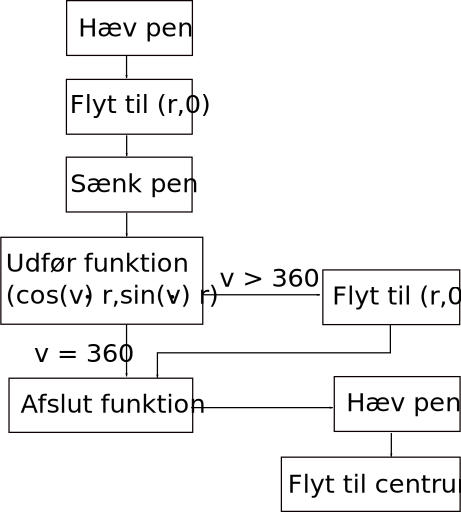
\includegraphics[width=0.5\textwidth]{./img/afviklingsdiagram-cirkel}
  \caption{Afviklingsdiagram for cirkelplot}
  \label{fig:hpgl-cirkel-afvikling}
\end{figure}


\section[Motorkontrol (med buffer)]{Motorkontrol}

% Hvordan er motorkontrollen implementeret? Beskriv implementeringen
% kort.



\begin{figure}[htbp]
  \centering
  
\includegraphics[width=.75\textwidth]{./img/la-behandling}
  \caption{Afviklingsdiagram over afvikling af LA-instruktionen.}
  \label{fig:la-behandling}
\end{figure}


\section{Stepmotorstyring}

% Hvordan styres stepmotorerne? Superkort. Hvordan ser softwaren der
% styrer dem ud?


\section{Sensorer og løfter/sænker}


%%% Local Variables: 
%%% mode: latex
%%% TeX-master: "../master"
%%% End: 

\backmatter

\chapter{Afslutning}
\label{ch:afslutning}

% Note om hvad der skal stå i dette afsnit her.  Fik vi opfyldt de
% overordnede produktkrav og vores egen kravspecifikation? Kom
% produktet til at virke?



%%% Local Variables: 
%%% mode: latex
%%% TeX-master: "../master"
%%% End: 

\listoffigures

\listoftables

\listoffixmes

\end{document}
